\chapter{System Analysis}

From the mathematical models, system analysis is performed in order to determine their behavior in time and frequency domains. Because control systems are then used on these dynamic states of the system to control their stability, steady-state error, tracking etc., among various others once the behavior in time and frequency domains are established.

\section{Time-domain analysis}

Time-domain analysis is response of the state of the dynamic system in time when given an input. The history of the response of the dynamic state due to the input is plotted as the time-response of the system. 

As dynamic systems are modeled using ODE's, their response can be determined using integration over a certain period of time either analytically or numerically. The time response of a LTI system consists of \textbf{transient response} and \textbf{steady-state response} due to an input to the system. These responses correspond to the null solution and the particular solution of the governing differential equation \cite{CTMS2019_Analysis}.

\section{Frequency domain analysis}

LTI systems have a property such that for any signaled input to the system, the output is also with the same frequency but could vary in phase and magnitude. This difference in phase and magnitude is the function of the input frequency and hence such response corresponds to the frequency response of the system \cite{CTMS2019_Analysis}.

In order to find the frequency response of the system, first the transfer function of the system is derived. Then using the complex variable $s$, the values of the plant transfer function is derived at every frequency starting from ($0$ to $\infty$). Here, $s$ is given by $s = \sigma \pm j \omega$, $\sigma$ is the real part of the root and indicates the damping in the system, $j \omega$ terms that lie on the imaginary  axis indicates the frequency of the system's oscillation. Therefore, by substituting $G(s) = G(j \omega)$ ($s = j \omega$), a frequency response of the system can be studied. If $G(s)$ is the open-loop transfer function of the system and $\omega$ is the vector of input frequencies, then the frequency response can be evaluated for every $\omega$ \cite{CTMS2019_Analysis}.

With the transfer function $G(s)$, the frequency response of the function $G(s)$ can be derived for every $s = j \omega$ and a plot of output $G(j\omega)$ versus input frequencies $\omega$ is plotted which is called \textbf{\textit{Bode Plot}}. Since $s$ is in complex plane both the magnitude and the phase of output frequencies $G(j\omega)$ can be plotted using \textbf{\textit{Bode Plot}}. As well as the position of $G(j\omega)$ in the complex plane can be studied using \textbf{\textit{Nyquist Diagrams}} \cite{CTMS2019_Analysis}.

\section{Analysis of first order systems}

A first order system hereby called PT-1 systems can be expressed in their most general form as:

\begin{equation} \label{Eq_PT1}
	\tau \dot{y}(t) + y(t) = k_{dc} u (t)
\end{equation}

Where $\tau$ and $k_{dc}$ are the parameters of the system or the constant coefficients of ODE. $k_{dc}$ is the amount of scaling of the systems output for a constant input. $\tau$ defines the amount of time required for the system to obtain $63.2 \%$ of the transient dynamics that the system undergoes. It is easier to determine the solutions of the equation \eqref{Eq_PT1} in algebraic form, \eqref{Eq_PT1} is written in the Laplace domain as:

\begin{equation} \label{Eq_PT1_TF}
	G(s) = \frac{Y(s)}{U(s)} = \frac{k_{dc}}{\tau s + 1}
\end{equation}

Again, where, $\tau$ and $k_{dc}$ are the parameters that completely define the response characteristics of a first order system and are called time constant and DC gain respectively. A time response of a PT-1 system is described using time signals such as step or impulse as inputs.

From equation \eqref{Eq_PT1_TF}, the denominator values of $s$ for which the equation goes to infinity is called the pole (values) of the system given by equation \eqref{Eq_PT1_TF}. In equation \eqref{Eq_PT1_TF}, we have only one possible value of $s$ at $s = -1/\tau$. Such a system with one pole is also defined as a first order system. Similarly a second order system will have two poles \cite[t.2.05]{RickHill_11}.

\subsection{Impulse response}

Consider a unit impulse as input to the first order system. The Laplace transform of the impulse signal is given by $L(s) = 1$. Therefore, the first order system with an impulse input is expressed as:
\begin{equation} \label{Eq_PT1_Impulse}
Y(s) = G(s)U(s) = \frac{k}{\tau s + 1} \cdot 1
\end{equation}
the inverse Laplace of the equation \eqref{Eq_PT1_Impulse} will express the solution of the equation of the differential equation \eqref{Eq_PT1} with an unit impulse input:
\begin{equation} \label{Eq:FirstOrderImpulseRespose}
y(t) = \frac{k}{\tau}e^{-\frac{t}{\tau}}
\end{equation}
The above equation is the null solution of the differential equation \eqref{Eq_PT1} given as $y = C e^{at}$ with initial condition $C = k/\tau$ and $a = -1/\tau$. From the solution \eqref{Eq:FirstOrderImpulseRespose} it can be inferred that for an unit impulse, the response of the system at time $t = \infty$ is to settle down to zero with an exponential decay. From a numerical solution generated in MATLAB, the response decays to zero as shown in figure \ref{fig:ImpulseReponseFirstOrderSystem}.
\begin{figure}[h!]
	\centering
	\includegraphics[scale=0.6]{Bilder/ImpulseReponseFirstOrderSystem.pdf}
	\caption{Impulse response of a first order system}
	\label{fig:ImpulseReponseFirstOrderSystem}
\end{figure}

\subsection{General first order responses}

A PT-1 system is first expressed in time-constant form as given below:
\begin{equation}
	\tau \frac{dy(t)}{dt} + y(t) = K u(t)
\end{equation}
where $y(t)$ and $u(t)$ are the state and inputs of the system respectively. The behavior of the system given by the above equation is described for $t > 0$ for various inputs $u(t)$ and / or initial conditions. The behavior is focused on how the output $y(t)$ changes with time constant $\tau$.

A time constant $\tau$ is defined for a more general system described by constant coefficients:
\begin{equation}
	a \frac{dy(t)}{dt} + b y(t) = c u(t)
\end{equation}
writing the above equation in time-constant form is to write the equation with coefficients of $y(t) = 1$. In such a case, the following operation is performed:
\begin{equation}
	\frac{a}{b} \frac{dy(t)}{dt} + y(t) = \frac{c}{b} u(t)
\end{equation}
therefore, the time-constant is defined by the ratio $a/b$, using the constant coefficients of PT-1 system. The ratio $a/b$ appears along with time variable $t$ in the solution of PT-1 systems and therefore serves as a factor to split and measure time, which is used to measure the system output at those factored times.

Similarly, the gain of the system is defined using the ratio $c/b$, as this appears as the coefficient of $u(t)$, it is the scaling of $y(t)$ for the given input $u(t)$. Therefore, the ratio $c/b$ is defined the gain of the system.

\subsubsection{$u(t) = 0$, non-zero initial condition}

\begin{equation}
	\tau \frac{dy}{dt} + y = 0 \implies y(t) = y(0) e^{-1/\tau}
\end{equation}

The solution shown above can be verified using LT:

\begin{equation}
	\implies \tau [s Y(s) - y(0)] + Y(s) = 0 \implies [s \tau + 1] Y(s) - \tau y(0) = 0
\end{equation}

Rearranging the above equation:
\begin{equation} \label{Eq_PT1_nonzeroICResponse}
	Y(s) = \frac{\tau y(0)}{s \tau + 1} = \frac{y(0)}{s + 1/\tau} \implies y(t) = y(0) e^{-t/\tau}
\end{equation}

These responses are characterized primarily by time-constant, which are the results derived from the solution:

\begin{enumerate}
	\item if $t = \tau$, $\implies y(t) = y(0) e^{-1} = 0.37 y(0)$
	\item if $t = 2\tau$, $\implies y(t) = y(0) e^{-2} = 0.14 y(0)$
	\item if $t = 3 \tau$, $\implies y(t) = y(0) e^{-3} = 0.05 y(0)$
	\item if $t = 4 \tau$, $\implies y(t) = y(0) e^{-4} = 0.02 y(0)$
\end{enumerate}

summary of responses:

\begin{table}[h!]
	\begin{tabular}{m{4cm} m{4cm} m{6cm}}
		\toprule
		\textbf{time} & \textbf{e} & \textbf{response} \\
		\cmidrule{1-3}
		$t = \tau$ & $e^{-1}$ & 37 $\%$ of initial condition \\
		$t = 2 \tau$ & $e^{-2}$ & 14 $\%$ of initial condition \\
		$t = 3 \tau$ & $e^{-3}$ & 5 $\%$ of initial condition \\
		$t = 4 \tau$ & $e^{-4}$ & 2 $\%$ of initial condition \\
		\bottomrule
	\end{tabular}
	\caption{Table summarizing PT-1 response for non-zero initial conditions}
\end{table}

\subsubsection{Step response}

The object is to find the solution to the differential equation $y(t)$ as given by the equation \eqref{Eq_PT1}. This system with a unit step input $u(t) = 1$ can be expressed in the Laplace domain by multipliying the input signal as:
\begin{equation} \label{Eq_PT1_step}
Y(s) = G(s) U(s) = \frac{k}{\tau s + 1}\frac{1}{s}
\end{equation}

Taking the inverse Laplace transform of equation \eqref{Eq_PT1_step}, the algebraic solution of the ODE given by equation \eqref{Eq_PT1} can be expressed as:

\begin{equation}\label{Eq_PT1_stepResponse}
y(t) = k - k e^{-t/\tau}
\end{equation}
The solution of the PT-1 system should have both null and particular solutions. The term with exponential function was initially assumed response of a homogeneous system. Therefore, the first term is the particular solution and the second term is the null solution of the ODE for PT-1 systems. In general, the terms of the null solution will impose the dynamics of the states in the system which decay after a while leaving behind the steady-state impact of the particular solution. The influence of the particular solution remains in the system as long as the input remains active without changing.

Further the stability of the system can be analyzed using \textbf{\textit{BIBO}} or using \textbf{\textit{Eigen value Analysis}}. Both the analyses lead to the same conclusion of system stability that do not blow up while operation. A BIBO stability can be performed numerically using MATLAB by choosing system parameters $\tau$ and $k_{dc}$ and a plot is generated as shown in figure \ref{fig:StepResponseFirstOrder}.
\begin{figure}[h!]
	\centering
	\includegraphics[scale=0.6]{Bilder/firstOrderSystemStepResponse.pdf}
	\caption{Step response of a first order system}
	\label{fig:StepResponseFirstOrder}
\end{figure}
Further analysis on system parameters can be made numerically such as the DC gain can be inferred from the steady-state value reached by the system. For a unit step input, the DC gain is given by the step-up value at which the output of the system's response settles down, in this case, $k = 5$ which is evident from the system value chosen to generate this plot. The time constant $\tau$ can be inferred from plot and equation \eqref{Eq_PT1_stepResponse}, for time $t = \tau$:
\begin{equation}
y(t) = k(1 - e^{-1}) = 0.632 k
\end{equation}
therefore, at one time constant $\tau$, the systems response settles down to about $63.2\%$ of the steady-state vale. Generally, a steady-state response is fixed when this value reaches $98\%$ of steady-state value, which from the plot and equation \eqref{Eq_PT1_stepResponse} can be inferred as at time $t = 4 \tau$:
\begin{equation}
y(t) = k(1 - e^{-4}) = 0.98 k
\end{equation}

Summary of PT-1 systems step response:

\begin{table}[h!]
	\centering
	\begin{tabular}{m{2cm} m{2cm} m{4cm}}
		\toprule
		\textbf{time} & \textbf{e} & \textbf{response} \\
		\cmidrule{1-3}
		$t = \tau$ & $(1 - e^{-1})$ & 63 $\%$ of steady-state response \\
		$t = 2 \tau$ & $(1 - e^{-2})$ & 84 $\%$ of steady-state response \\
		$t = 3 \tau$ & $(1 - e^{-3})$ & 95 $\%$ of steady-state response \\
		$t = 4 \tau$ & $(1 - e^{-4})$ & 98 $\%$ of steady-state response \\
		\bottomrule
	\end{tabular}
	\caption{Table summarizing step response of PT-1 system}
\end{table}

\subsubsection{step response with non-zero initial condition}

For a linear system, the response due to two different inputs can be determined using principle of superposition. Since we already now the response from step input and non-zero initial condition, they both can just be added together. Therefore, from equations \eqref{Eq_PT1_nonzeroICResponse} and \eqref{Eq_PT1_stepResponse}, we have:

\begin{equation} \label{Eq_PT1_stepAndICresponse}
	y(t) = y(0) e^{-t/\tau} + K (1 - e^{-t/\tau}) = (y(0) - K) e^{-t/\tau} + K
\end{equation}

The term $(y(0) - K) e^{-t/\tau}$ in equation \eqref{Eq_PT1_stepAndICresponse} gives the exponential decay from the IC and ss-response $K$ from step input.

The above response can also be derived using LT, by putting both LT's for IC and step-function into the equation of PT-1 system:
\begin{equation}
	[s \tau + 1] Y(s) - \tau y(0) = \frac{K}{s}
\end{equation}
then solving the above equation for $Y(s)$ and doing inverse LT, the solution can be derived.

Observations made from the solution: Consider the response given by equation \eqref{Eq_PT1_stepAndICresponse}, the following observations can be made:
\begin{enumerate}
	\item ss: depends on the gain $K$ and the input of the system. Therefore, ss = $K$
	\item Dynamics: depend on how fast the exponential goes to zero, this depends solely on the time constant $\tau$
	\item The term $(y(0) - K)$ in equation \eqref{Eq_PT1_stepAndICresponse} defines the distance from IC to the ss
\end{enumerate}

The response by changing $\tau$, let $(y(0) - K) = d$:

\begin{table}[h!]
	\centering
	\begin{tabular}{m{2cm} m{2cm} m{3cm} m{5cm}}
		\toprule
		\textbf{time} & \textbf{d}  & \textbf{y(t)} & \textbf{response} \\
		\cmidrule{1-4}
		\cmidrule{1-4}
		$t = 0$ & $ y(0) - K $ & $y = K + d = y(0)$ & At the initial state \\ \cmidrule{1-4}
		$t =  \tau$ & $ 0.37(y(0) - K) $ & $y = K + 0.37d$ & 37 $\%$ deviation from ss \\ \cmidrule{1-4}
		$t = 2 \tau$ & $ 0.14(y(0) - K) $ & $y = K + 0.14d$ & 14 $\%$ deviation from ss \\ \cmidrule{1-4}
		$t = 3 \tau$ & $ 0.05(y(0) - K) $ & $y = K + 0.05d$ & 5 $\%$ deviation from ss \\
		\bottomrule
	\end{tabular}
	\caption{Table summarizing response of PT-1 due to step input and IC}
\end{table}

From the list and the able given above, it seems that for PT-1 systems, with step input and non-zero IC, the system starts from IC and ends at ss. Where IC = $Y(0)$ and ss = $K$. 

consider an example PT-1 system:
\begin{equation}
	2 \frac{dy}{dt} + 6 y = 4 u
\end{equation}

writing in time-constant form:

\begin{equation}
	\frac{1}{3} \frac{dy}{dt} + y = \frac{2}{3} u \quad @ \quad y(0) = -1
\end{equation}

Before, generating the plot, the following observations can be made by comparing to the standard response:
\begin{itemize}
	\item $\tau = 1/3$ and $K = 2/3$
	\item at $t = 0$ response starts at $y(0) = -1$ at a distance $d = y(0) - K$ and ends at ss = $K = 2/3$ when $t > 3 \tau$
	\item for a ss of 5 $\%$, simulation time should run upto $t = 3 \tau$
\end{itemize}

\section{Stability analysis of PT-2 systems}

% For simple systems such as a rectangular cube, a clear distinction can be made easily between its equilibrium and stability states. Such that, the rotation about its principal axes is always at equilibrium, but for any perturbation, stability is guaranteed only for two among the three principal axes. However, for complex systems such as a bicycle, defining equilibrium points and stable states are more complicated. 
Once a model of a system has been established, it may be required to analyze the model in order to determine the response of the system, in this case in the time domain. In the perspective of a control design, the control system is often designed to improve the stability of the system, improve the speed of the response or the steady-state error, or prevent oscillations. Therefore, it is necessary to determine the dynamic properties of the system from the system model.
In this section, stability is defined formally for linear and non-linear systems (such as a bicycle).

\subsection{Stability in linear systems} \label{Sec_StabilityLinearSystems}

For defining the important concepts in stability analysis, a simple second order linear and homogeneous system is considered as described below:
\begin{equation} \label{Eq_SecondOrderSystem}
\Ddot{y} + B \Dot{y} + C y = 0
\end{equation}
For a special case (roots of characteristic equation lie in complex $s$ plane) such that the solution of the above ODE is given by $y = e^{st}$, the above ODE can be re-written into its characteristic algebraic form by substituting $y = e^{st}$:
\begin{equation} \label{Eq_CharacteristicEquationPT2}
s^2 + B s + C = 0
\end{equation}
the roots of the above equation are given by:
\begin{equation}
\{s_1,s_2\} = \frac{-B \pm \sqrt{B^2 - 4 C}}{2}
\end{equation}
and the null (homogeneous) solution of the equation \eqref{Eq_CharacteristicEquationPT2} can be expressed as the linear combination of roots:
\begin{equation} \label{Eq_GS_Char_PT2}
y(t) = C_1 e^{s_{1}t} + C_2 e^{s_{2}t}
\end{equation}
Alternatively, writing equation \eqref{Eq_SecondOrderSystem} in a general state equation matrix form (two first orders):
\begin{equation}
\frac{d}{dt} \begin{bmatrix}
	y \\ y^{\prime}
\end{bmatrix} = \begin{bmatrix}0 & 1 \\
-C & -B\end{bmatrix} \begin{bmatrix}y \\ y'\end{bmatrix}
\end{equation}
alternatively, the above equation can be realized in the form:
\begin{equation}
\frac{d}{dt}\vec{Z} = \begin{bmatrix} \vec{A} \end{bmatrix} \begin{bmatrix} \vec{Z} \end{bmatrix}
\end{equation}
where $\vec{Z}$ is the state matrix $[y \quad y^{\prime}]^{T}$, $\vec{A}$ is called the companion matrix (also system matrix for the dynamic states $\vec{Z}$), matrix $\vec{A}$ can be used to find the Eigen-Values of $\vec{A}$:
\begin{equation}
\{\lambda_1,\lambda_2\} = \frac{-B \pm \sqrt{B^2 - 4 C}}{2}
\end{equation}
and the null solution of the second order differential equation:
\begin{equation}
y(t) = C_1 e^{\lambda_{1}t} + C_2 e^{\lambda_{2}t}
\end{equation}
Both the null solutions predicted by the roots $\{s_1,s_2\}$ and Eigen-Values $\{\lambda_1,\lambda_2\}$ give the solution of the differential equation \eqref{Eq_SecondOrderSystem}, however, with Eigen-values it is much easier to reach at the null solution. %as the problem now is transformed from differential calculus to linear algebra.
From the roots $\{s_1,s_2\}$ or the Eigen-Values $\{\lambda_1,\lambda_2\}$, following cases can be drawn about the stability of the second order system:

\begin{table*}[h!] \centering
	\begin{tabular}{ccc}
		\toprule
		Cases & Condition & Eigen-Values \\ \hline 
		\\
		Over-damped & $(B^2 > 4 C)$ & Negative distinct Roots \\
		Critically damped & $(B^2 = 4 C)$ & Negative repeated roots \\
		Under-damped & $(B^2 < 4 C)$ & Complex conjugate roots \\
		Undamped & $B = 0$ & Imaginary Roots \\
		\bottomrule
	\end{tabular}
	\label{Tab_PT2_Char_Roots}
\end{table*}

Since the characteristic equation \eqref{Eq_CharacteristicEquationPT2} is quadratic in nature, the roots will be of complex in nature. With complex roots it can be said that the imaginary part will indicate the frequency of systems oscillations and the real part will indicate the damping (or growth based on parameter $B$) of the system. In case of undamped system, even the BIBO stability can not be said to be achieved completely as the system will be oscillating with an undamped magnitude (high risk of resonance). Therefore, the BIBO and the asymptotic stability of the system can only be defined in the cases where there is a damping \cite{RickHill_11}.

In terms of BIBO stability the stability of the PT-2 system can be roughly described using the values of the real part and can be described as follows:
\begin{itemize}
	\item Pure oscillations: Real part of poles is zero.
	\item Exponential decay (BIBO stability): Real part are negative.
	\item Exponential growth (unstable): If at-least one of the Real part is positive.
\end{itemize}

\textbf{Asymptotic stability}: The PT-2 system is considered to be asymptotically stable if and only if, the state $x \rightarrow 0$ as $t \rightarrow \infty$ \cite[t.8.45]{RickHill_11}.

\textbf{BIBO stability}: A system is said to be BIBO stable if for any bounded inputs the system outputs remain bounded ie., the system output does not blow up.

For linear systems, using these two stability criterion the stability of PT-2 system can be established.

\subsection{Stability Analysis in Non-linear systems} \label{Sec:StabilityNonLinearSystems}

With linear systems, if the system is already in the stable condition, then regardless of the initial conditions, the system will get back to its stable position. However, a non-linear system is stable only if the perturbations lie within a certain range of neighborhood. Lets consider a non-linear autonomous system (time-invariant system) expressed as a first order system dependent on velocity:
\begin{equation}
\Dot{x} = f(x)
\end{equation}
The equilibrium states can be defined for a non-liner system if it satisfies the condition:
\begin{equation}
\Dot{x} = f(x_{e}) = 0 \quad \forall t > t_0
\end{equation}
where $x_e$ is the point at which the function $f(x) = 0$ and $x_e = constant$. The neighborhood is defined as: Given perturbation $\delta > 0$, a state vector $x(t)$ is said to be in the neighborhood $B_b(x_r(t))$ of the state $x_r(t)$ if:
\begin{equation}
\norm{x(t) - x_r(t)} < \delta
\end{equation}
then,
\begin{equation}
x(t) \quad \in \quad B_{\delta}(x_r(t))
\end{equation}

\begin{figure}[h!]
	\centering
	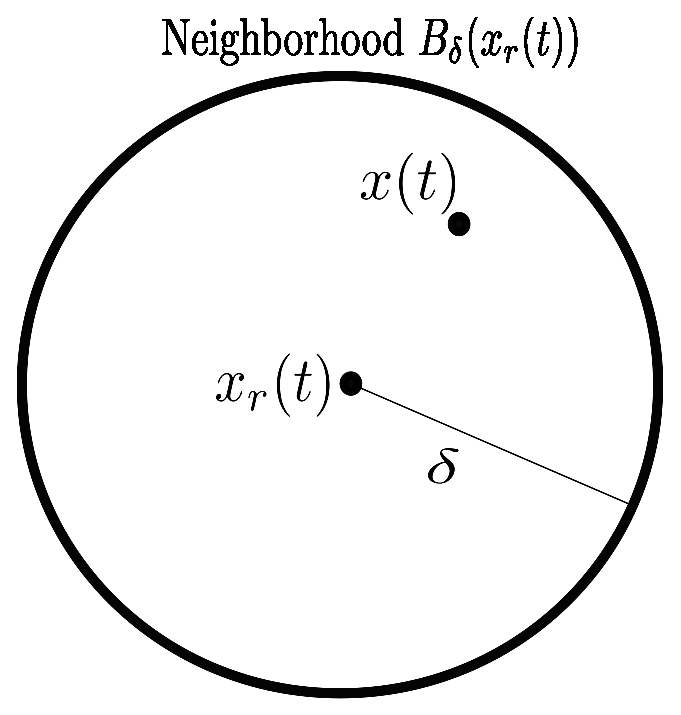
\includegraphics[scale=0.5]{Bilder/Neighborhood.eps}
	\caption{Neighborhood of a non-linear system stability}
	\label{fig:Neighborhood}
\end{figure}

\textbf{\textit{Lagrange stability}} is defined as: the state $x(t)$ is said to be Lagrange stable (or bounded) relative to $x_r(t)$ if there exists a $\delta > 0$ such that:
\begin{equation}
x(t) \quad \in \quad B_{\delta}(x_r(t)) \quad \forall t > t_0
\end{equation}

\begin{figure}[h!]
	\centering
	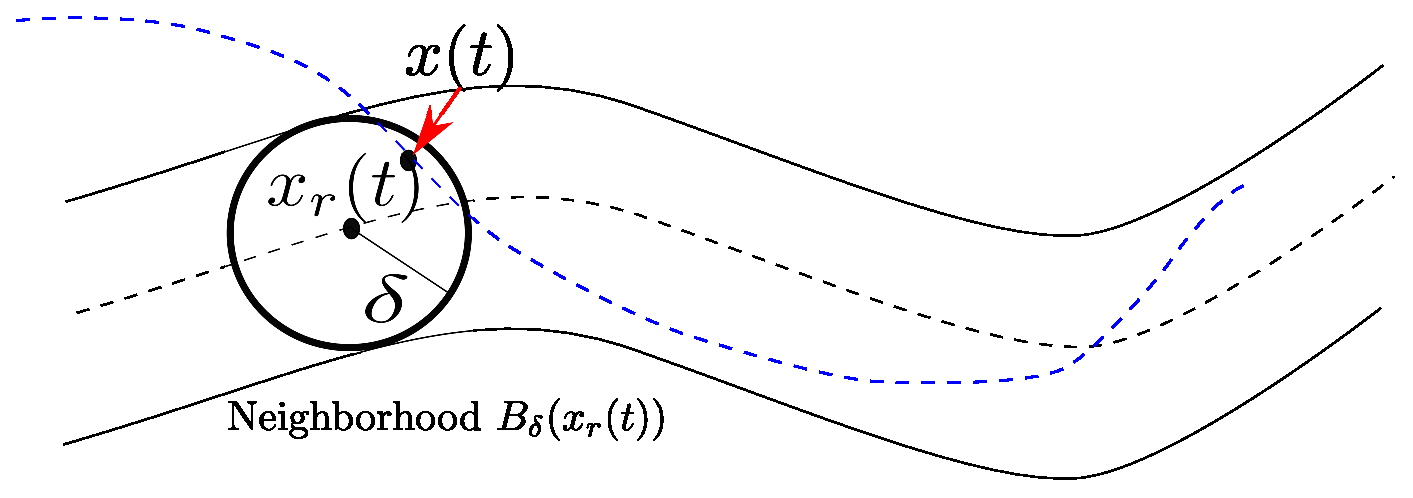
\includegraphics[scale=0.5]{Bilder/LagrangeStability.eps}
	\caption{Lagrange Stability}
	\label{fig:LagrangeStability}
\end{figure}

\textbf{\textit{Lyaponov stability}} of non-linear system is defined as: the state $x(t)$ is said to be Lyaponov stable relative to $x_r(t)$ if for each $\epsilon > 0$ there exists a $\delta(\epsilon)>0$ such that:
\begin{align}
x(t_0) \quad &\in \quad B_{\delta}(x_r(t_0)) \\
x(t) \quad &\in \quad B_{\epsilon}(x_r(t)) \quad \forall t > t_0
\end{align}
Unlike Lagrange stability, in Lyaponov stability lets to define another neighborhood $B_{\epsilon}(x_r(t))$ such that perturbations in the previous neighborhood $B_{\delta}(x_r(t_0))$ would lead to $B_{\epsilon}(x_r(t))$, hence, unlike Lagrange stability which does not depend on the initial conditions (but on the physics of the problem) Lyaponov stability narrows down the initial states that could lead to stability in the motion in a later state. Also, unlike in the linear systems, the non-linear systems would lead to convergence just because the system is in the stable condition. The boundary $B_{\epsilon}(x_r(t))$ could be very close to $B_{\delta}(x_r(t_0))$ and the system would be stable in the $\epsilon$. For numerical simulation, it is required that the simulations are run for long enough time to prove that the stability remains within the conditions described by the Lyaponov conditions.

\begin{figure}[h!]
	\centering
	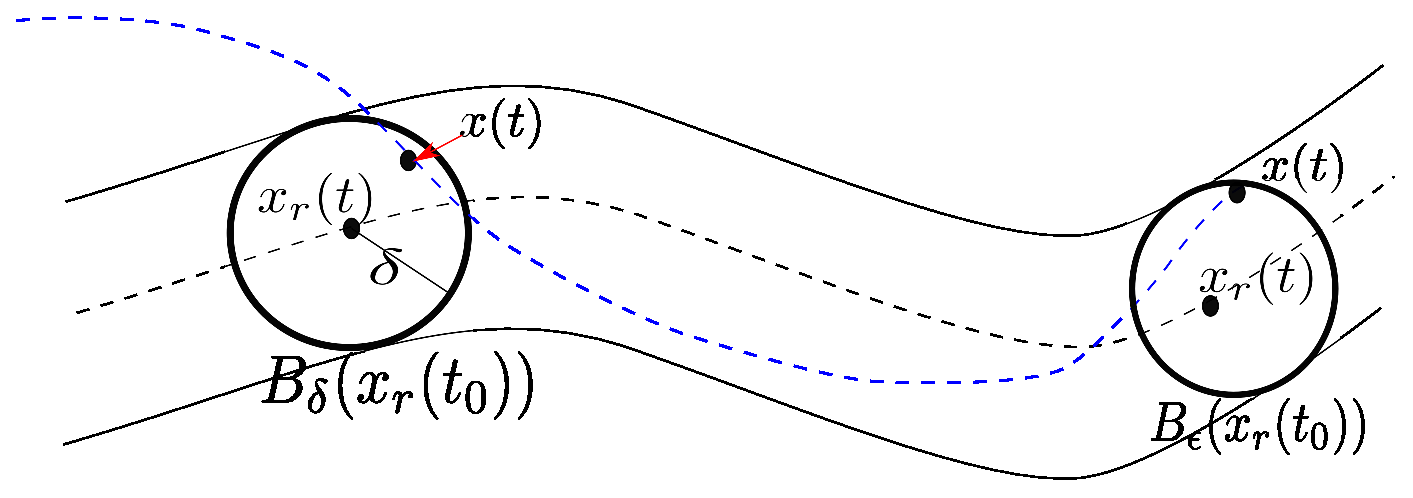
\includegraphics[scale=0.5]{Bilder/LyaponovStability.eps}
	\caption{Lyaponov Stability}
	\label{fig:LyaponovStability}
\end{figure}

Once Lyaponov stability has been defined, an \textbf{\textit{Asymptotic stability}} can be extended and defined as: the state $x(t)$ is asymptotically stable relative to $x_r(t)$ if $x(t)$ is Lyaponov stable and there exists a $\delta > 0$ such that:
\begin{align}
x_0(t) \quad &\in \quad B_{\delta}(x_r(t_0)) \quad \text{then,}\\
\lim_{t\to\infty} x(t) \quad &= \quad x_r(t)
\end{align}
\begin{figure}[h!]
	\centering
	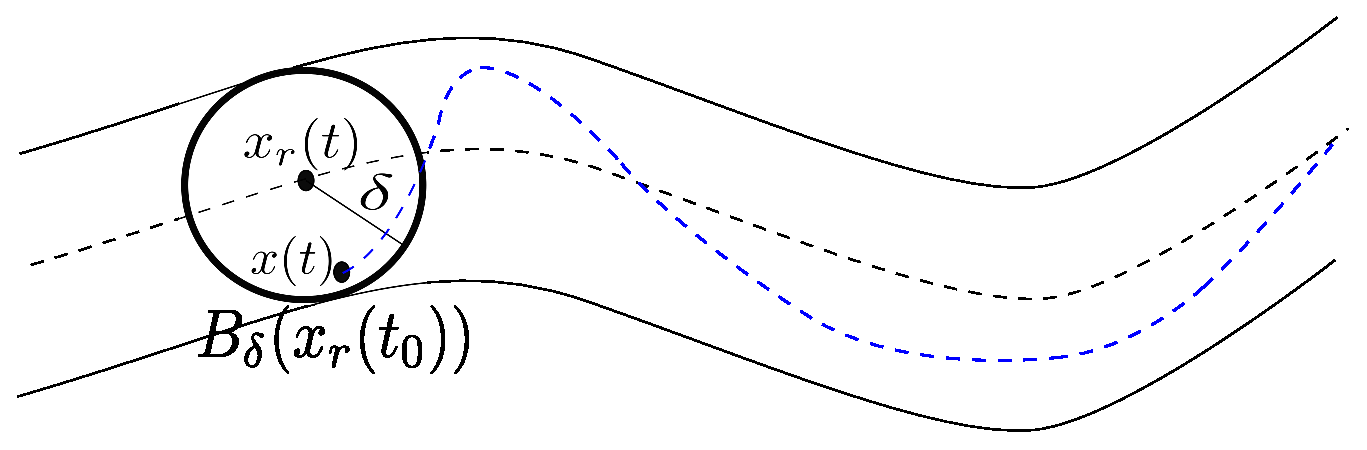
\includegraphics[scale=0.5]{Bilder/AsymptoticStability.eps}
	\caption{Asymptotic stability}
	\label{fig:AsymptoticStability}
\end{figure}
Therefore, in case of asymptotic stability, the boundary due to $\epsilon$ goes to zero and the boundary $B_{\epsilon}(x_r(t))$ does not exists anymore, so now the motion $x(t)$ converges to the reference $x_r(t)$. This is an ideal condition to converge to from controls perspective. Certain dynamic systems have shown to converge to this stability point in their natural modes of operation. A bicycle is one such example where under a certain range of velocities the weave motion of the bicycle converges to asymptotic stability by damping (not physically damping like in friction) the weave motion towards a zero lean and steering rates. 

\subsection{Solving / Analysing PT-2 using Laplace transform} \label{Sec_Solving_PT2_Laplace}

Laplace transform of the PT-2 system can be expressed as:
\begin{equation}\label{Eq_Laplace_PT2}
G(s) = \frac{Y(s)}{U(s)} = \frac{\omega_{n}^{2}}{s^{2} + 2 \zeta \omega_{n} s + \omega_{n}^{2}}
\end{equation}
the poles of the denominator in equation \eqref{Eq_Laplace_PT2} can be found:
\begin{equation*}
s_{1,2} = \frac{-2 \zeta \omega_{n} \pm \sqrt{4 \zeta^{2} \omega_{n}^2 - 4 \omega_{n}^2}}{2} = -\zeta \omega_{n} \pm \omega_{n} \sqrt{\zeta^2 - 1} = -\zeta \omega_{n} \pm j \omega_{n} \sqrt{1 - \zeta^2}
\end{equation*}

with poles $s_{1,2} = -\zeta \omega_{n} \pm j \omega_{n} \sqrt{1 - \zeta^2}$, the stability analysis of the system can be made based on the numerical values of the roots. Only $\zeta$ is a variable and $\omega_{n}$ is a constant also $\zeta$ can be controlled as a variable as the system frequency $\omega$ varies. Therefore, $\zeta$ now becomes the fundamental variable for the behavioral changes in the motion as follows:
\begin{table}[h!]
	\centering
	\begin{tabular}{m{4em} m{8em} m{8em}}
		\toprule
		$\zeta = 0$ & poles are Im  & undamped \\
		$\zeta < 1$ & poles are complex & under-damped \\
		$\zeta = 1$ & repeated real poles & critically damped \\
		$\zeta > 1$ & distinct real poles & over damped \\ \bottomrule
	\end{tabular}
\end{table}
\begin{figure}[h!]
	\centering
	\includegraphics[width=\linewidth]{Bilder/Poles_PT2_system}
	\caption{Poles in the PT2 system}
\end{figure}

\subsubsection{Determining the system behavior} \label{Sec_PT2_system_properties}

Various system behaviours can be determined using the resuts from the previous analysis and they are important which define the PT-2 systems acording to their behavior. Using an underdamped system response various system behaviors can be defined as with underdamped systems all the system behaviorial characteristics are clearly visible. Using Laplace transforms with a step function the solution of PT-2 system can be found using inverse Laplace as shown in the red box in figure \ref{Fig_Sol_PT2_StepInput_Laplace}.
\begin{figure}[h!]
	\centering
	\includegraphics[width=\linewidth]{Bilder/Sol_PT2}
	\caption{Solution to PT-2 system with step input using Laplace transform}
	\label{Fig_Sol_PT2_StepInput_Laplace}
\end{figure}
Several important properties highlighted by the solution obtained in figure \ref{Fig_Sol_PT2_StepInput_Laplace} can be seen visually as shown in figure \ref{Fig_Prop_PT2_Laplace}.
\clearpage
\begin{figure}[h!]
	\centering
	\includegraphics[width=\linewidth]{Bilder/Prop_PT2}
	\caption{Important behvarial propertial seen in PT-2 systems}
	\label{Fig_Prop_PT2_Laplace}
\end{figure}
These important properties can be listed as follows:
\begin{enumerate}
	\item Delay time
	\item Rise time
	\item Settling time
	\item Peak time
	\item Maximum Overshoot
\end{enumerate}
the definitions and analytical deduction of the properties are given in figures (\ref{Fig_Delay_and_Rise_PT2_Laplace}, \ref{Settling_time_PT2}, \ref{Peak_time_PT2} and \ref{Max_overshoot_PT2}).
\begin{figure}[h!]
	\centering
	\includegraphics[width=\linewidth]{Bilder/Delay_and_Rise_time_PT2}
	\caption{Delay and Rise times seen in PT-2 systems}
	\label{Fig_Delay_and_Rise_PT2_Laplace}	
\end{figure}
\clearpage
\begin{figure}[h!]
	\centering
	\includegraphics[width=\linewidth]{Bilder/Settling_time}
	\caption{Settling time seen in PT-2 systems}
	\label{Settling_time_PT2}	
\end{figure}
Settling time is approximated by roughly determining the time required to settle down the state dynamics by 2\% at the steady state. The sinusoid inside the brackets will produce oscillations all the time unless they are completely damped out as $t \rightarrow \infty$. However by controlling the exponential value to reach $2\%$, the output from the sinosoids can be be controlled within $2\%$. Therefore, from the analogy that $e^{-4} \approx 0.02$, the settling time $t_s$ is approximated to $4 / \sigma$.
\begin{figure}[h!]
	\centering
	\includegraphics[width=\linewidth]{Bilder/Peak_time_PT2}
	\caption{Peak time seen in PT-2 systems}
	\label{Peak_time_PT2}	
\end{figure}
\begin{figure}[h!]
	\centering
	\includegraphics[width=\linewidth]{Bilder/Max_overshoot_PT2}
	\caption{Maximun overshoot seen in PT-2 systems}
	\label{Max_overshoot_PT2}	
\end{figure}

\clearpage

\subsection{Poles determine the system behavior} \label{Sec_PolesDetSysBehv}

Consider figure \ref{Fig_PolesSystemBehavior}, from the poles placed in the complex plane the following details can be extracted. The distance of the poles on the real axis is given by the real part of the roots and the distance of the poles on the imaginary axis is given by the Im part of the poles. The radius of the poles from the origin is defined by the natural frequency of the system $\omega_{n}$ and the angle between pole radius $\omega_{n}$ and real axis is given by $\beta$.
\begin{figure}[h!]
	\centering
	\includegraphics[width=\linewidth]{Bilder/PolesDetermineSysBehavior}
	\caption{Poles determine the system behavior}
	\label{Fig_PolesSystemBehavior}
\end{figure}

From the relationship $cos{\beta} = \zeta$ it can be said that the angle $\beta$ determines the damping in the system such as when $cos{\beta} = \pi/2$ then damping is zero and the system oscillates freely. When $cos{\beta} = 0$, the poles lie exactly on the real axis and also lie on one another (repeated poles), making the system critically damp. Therefore, as the angle $cos{\beta}$ increases towards $\pi/2$, the damping in the system decreases and vice-versa.

\subsection{Solving / Analysis PT-2 using characteristic polynomial}

The general form of PT-2 using a characteristic polynomial is given by equation \eqref{Eq_CharacteristicEquationPT2} (the coefficients in various forms may vary but they don't change the solution or the behavior as they are constants and treated differently in different approaches). From the table \ref{Tab_PT2_Char_Roots}, the roots of the polynomial can be used to define the systems damping and therefore its behavior. For the first analysis, consider case (1) in the table \ref{Tab_PT2_Char_Roots} for roots $B^{2} > 4C$ leading to definite negative roots which overcome the oscillations from the Im roots and therefore make the system over damped.

With the roots of the characteristic equation \eqref{Eq_CharacteristicEquationPT2} given by $\{s_1, s_2\}$, the general solution of equation \eqref{Eq_CharacteristicEquationPT2} can be expressed as the linear sum of the solution of each roots as given by:
\begin{equation}
	y(t) = A e^{s_{1}t} + B e^{s_{2}t}
\end{equation}
where $A$ and $B$ are constants which are determined using initial conditions which is same as equation \eqref{Eq_GS_Char_PT2} just with different coefficients. Now equation \eqref{Eq_GS_Char_PT2} gives the general solution for a homogeneous PT-2 given by \eqref{Eq_CharacteristicEquationPT2}. For the sake of analysis, lets use a step function and perform a time-domain analysis of PT-2 systems. Now equation \eqref{Eq_SecondOrderSystem} can be written for a step input as:
\begin{equation} \label{Eq_PT2_stepInput}
	a \ddot{y} + b \dot{y} + c = 1
\end{equation}
the 1 on RHS signifies the external step input, with initial conditions $x(0) = \dot{x}(0) = 0$. Therefore now the general solution to equation \eqref{Eq_PT2_stepInput} is given by:
\begin{equation} \label{Eq_GS_PT2_stepInput}
	y(t) = A e^{s_{1}t} + B e^{s_{2}t} + \frac{1}{c}
\end{equation}
$A$ and $B$ can be solved using initial condition's using $y(t)$ and $\dot{y}(t)$ leading to:
\begin{align*}
	\left(\frac{s_2}{s_1} - 1 \right) B &= \frac{1}{c} \\
	A &= \frac{-s_2}{s_1} B
\end{align*}
therefore, equation \eqref{Eq_GS_PT2_stepInput} becomes:
\begin{equation}
	y = \frac{1}{c} \left[ 1 + \left( \frac{1}{s_1 + s_2} (s_1 e^{s_{2}t} - s_2 e^{s_{1}t}) \right) \right]
\end{equation}
$c$ can be determined at the steady-state such that at steady state $\ddot{y} = \dot{y} = 0$ which leads to $c = 1$ in equation \eqref{Eq_SecondOrderSystem}.

\subsection{Numerical solution for PT-2 systems using Matlab}

For linear systems, Matlab has many inbuilt functions that can be used directly to determine the various system properties given in section \ref{Sec_PT2_system_properties}. It is only necessary to remember these properties rather than be able to solve them analytically. Control system toolbox in Matlab can be used to conveniently determine all these properties on a computer rather by solving with pen and paper as well plot results to see these properties graphically for understanding.

Using the command \textbf{\textit{linearSystemAnalyzer('step',G)}}, a figure shows in Matlab all the properties of a linear PT-2 system which are evaluated numerically.
